\documentclass[a4paper,10pt]{article}
\usepackage{amsmath}
\usepackage{graphicx}
\usepackage[margin=0.8in]{geometry}
\usepackage[compact]{titlesec}

\setlength{\parskip}{0pt} % 删除段落间距
\setlength{\parindent}{0em} % 删除段落缩进
\renewcommand{\baselinestretch}{0.9} % 压缩行间距

\begin{document}
\pagestyle{empty}

\section*{\centering Analysis of Key West Annual Mean Temperatures}

\subsection*{Objective and Hypotheses}
The objective is to evaluate whether there is a significant correlation between the years (\texttt{Year}) and the annual mean temperatures (\texttt{Temp}) of Key West, using permutation tests.

\begin{itemize}
    \item \(H_0\): There is no correlation between \texttt{Year} and \texttt{Temp}.
    \item \(H_1\): There is a significant correlation between \texttt{Year} and \texttt{Temp}.
\end{itemize}

\subsection*{Data Overview}
The dataset contains 100 observations with two variables: \textbf{Year}, representing the year of observation, and \textbf{Temp}, representing the annual mean temperature in degrees Celsius. The statistical analysis indicates that the average annual temperature is 25.31°C, with a standard deviation of 0.495°C.

\subsection*{Methods}
The Pearson correlation coefficient between \texttt{Year} and \texttt{Temp} was calculated as \( r_{\text{observed}} = 0.68 \). A permutation test with \( n_{\text{sim}} = 10,000 \) iterations was conducted by shuffling \texttt{Temp} while keeping \texttt{Year} fixed, generating a null distribution of correlation coefficients. The p-value was computed as:
\[
p = \frac{1}{n_{\text{sim}}} \sum_{i=1}^{n_{\text{sim}}} \mathbf{1}\{|r_{\text{random}, i}| \geq |r_{\text{observed}}|\},
\]
where \( r_{\text{random}, i} \) is the \( i \)-th random correlation, and \(\mathbf{1}\) is the indicator function that equals 1 if the condition is true and 0 otherwise.

Although $n_{\text{sim}} = 10,000$ was chosen for this analysis to balance computational cost and precision, it is worth noting that as $n_{\text{sim}} \to \infty$, the empirical p-value $p_{\text{sim}}$ converges to the true p-value $p$ according to the law of large numbers. By testing various values of $n_{\text{sim}}$ (e.g., 10, 100, 1000, 10,000, and beyond), it became evident that due to the large observed value of $r_{\text{observed}} = 0.68$, the empirical p-value $p_{\text{sim}}$ was consistently $0$. However, it remains important to emphasize that as $n_{\text{sim}}$ increases, the empirical p-value $p_{\text{sim}}$ will still theoretically converge to a fixed value as $n_{\text{sim}} \to \infty$. Furthermore, by the central limit theorem, $p_{\text{sim}}$ approximately follows a normal distribution:
\[
p_{\text{sim}} \sim N\left(p, \frac{p(1-p)}{n_{\text{sim}}}\right),
\]
where $p$ is the true p-value. As $n_{\text{sim}}$ increases, the variance $\frac{p(1-p)}{n_{\text{sim}}}$ decreases, resulting in a more precise estimate of the p-value. Thus, larger $n_{\text{sim}}$ values lead to greater accuracy, though diminishing returns may be observed beyond a certain point.


\begin{figure}[h!]
\centering
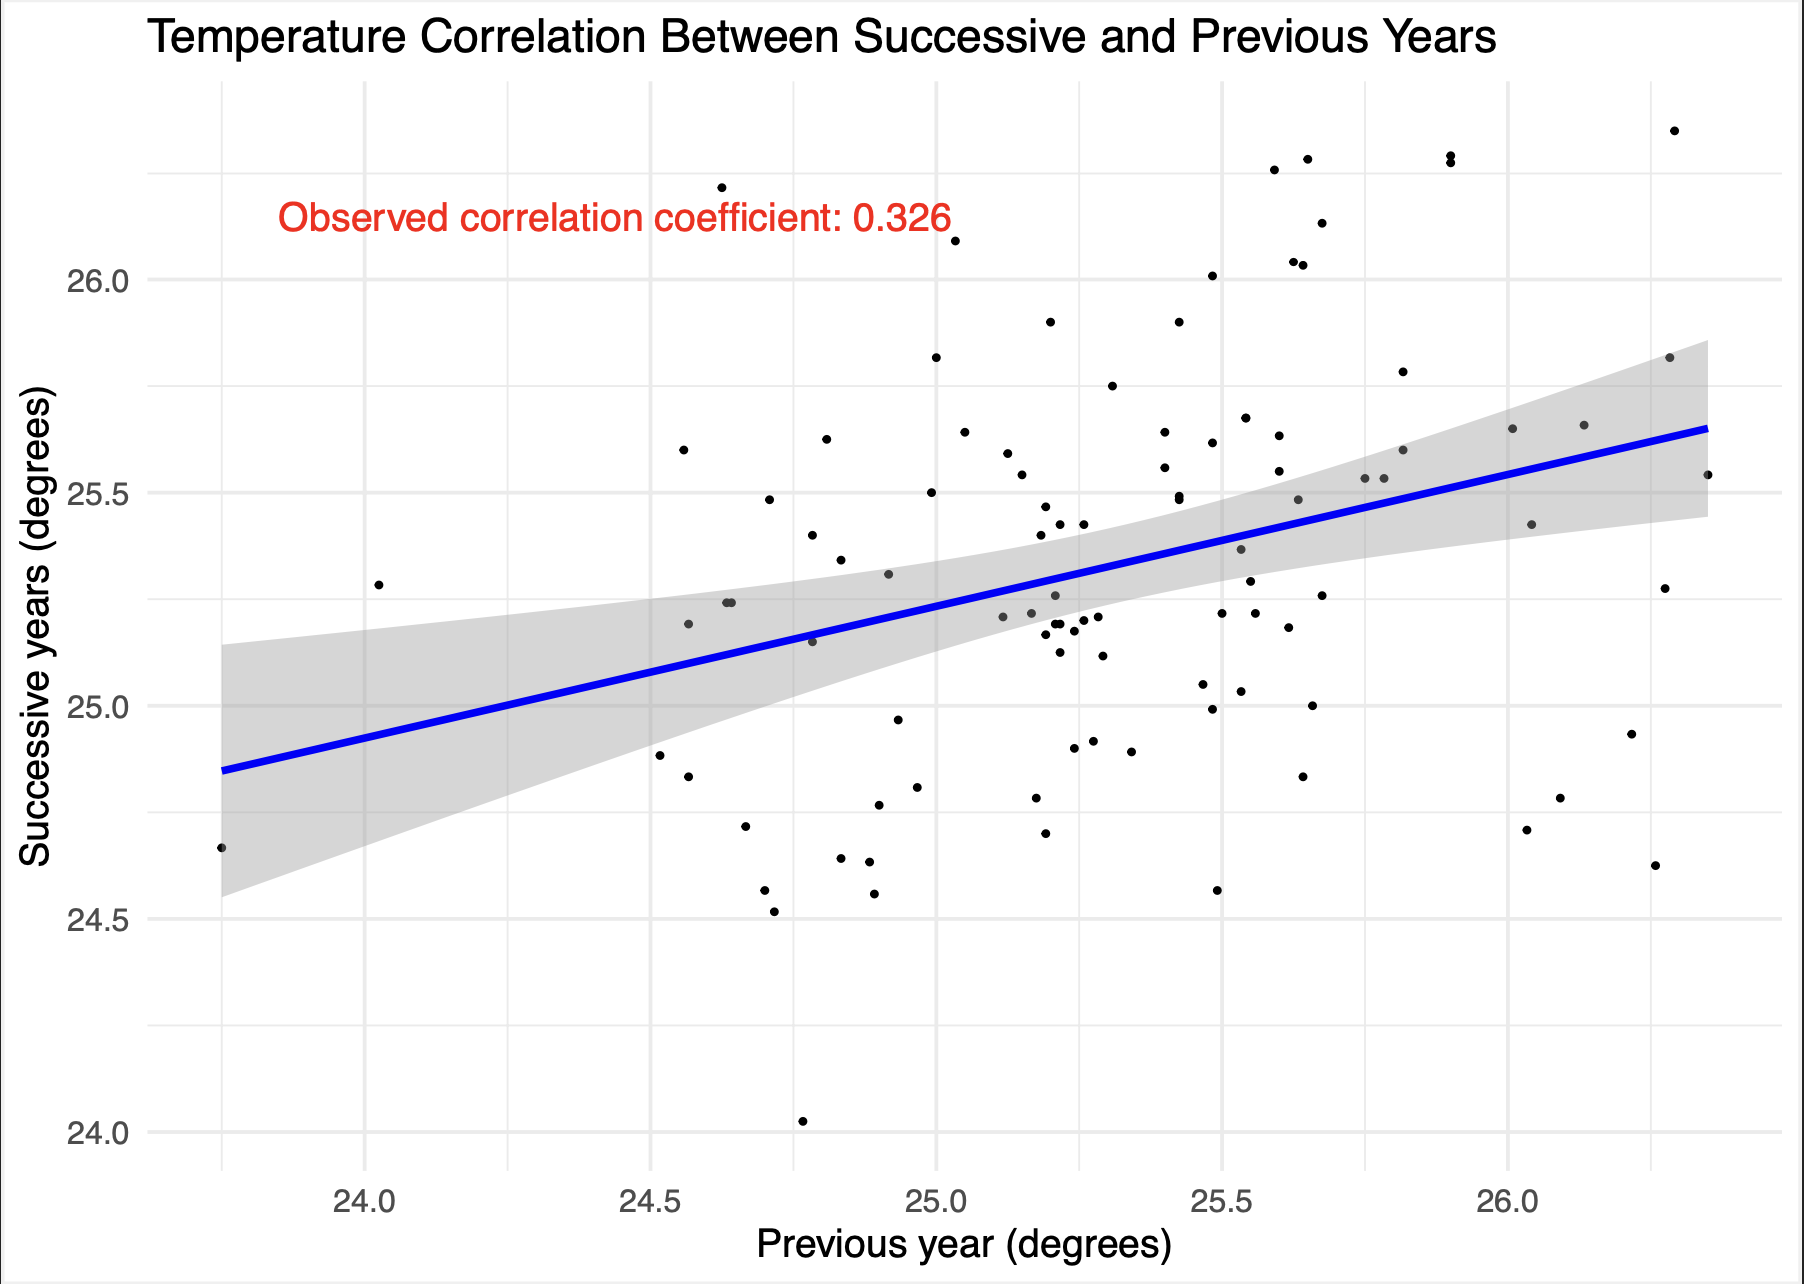
\includegraphics[width=0.45\textwidth]{../data/1.png}
\caption{Histogram of random correlation coefficients. Red dashed lines indicate the observed correlation.}
\label{fig:null_distribution}
\end{figure}

\subsection*{Results}
The observed Pearson correlation coefficient between \texttt{Year} and \texttt{Temp} was \( r_{\text{observed}} = 0.68 \). A permutation test with \( n_{\text{sim}} = 10,000 \) iterations yielded a p-value of \( p = 0 \), indicating that no random correlation coefficients in the null distribution were as extreme as the observed value.

Figure~\ref{fig:null_distribution} shows the null distribution of 10,000 random correlation coefficients, centered around 0. The red dashed lines represent the observed correlation \( r_{\text{observed}} = 0.68 \), which lies far in the tail, beyond any randomly generated values. This result strongly rejects the null hypothesis (\( H_0 \)), providing robust evidence of a significant positive relationship between \texttt{Year} and \texttt{Temp}. The observed correlation suggests a potential warming trend in Key West over time.

\end{document}
